
\documentclass[12pt]{report}

\usepackage{CJKutf8}
\usepackage{setspace}
\usepackage{CJK}
%\usepackage{pinyin}

%==
%\usepackage[active]{srcltx}
\usepackage[english]{babel}
\usepackage{amssymb,amsfonts,amsmath}
\usepackage{amsthm}
%\usepackage{fontspec}
\usepackage{mathrsfs}
\usepackage{bm}
\usepackage{url}
\usepackage{graphicx}
\usepackage{xcolor}
\usepackage{t1enc}
\usepackage{comment} 
\usepackage{makeidx}
\usepackage{xspace}
%==
\usepackage[a4paper,left=3cm,top=3cm,right=3cm,bottom=3cm,nohead]{geometry}
\setlength{\baselineskip}{10pt}
\DeclareMathAlphabet{\mathpzc}{OT1}{pzc}{m}{it}



%\renewcommand{\qed}{{ }\hfill$\Box$}

\newtheorem{conject}{Conjecture}


%\newcommand{\bin}{\ensuremath{\{0,1\}}}
\newcommand{\FM}{\ensuremath{FM}}

%---Lattice---

\newcommand{\latticeb}[1]{\ensuremath{\mathpzc{L} (\bm{#1})}}


% ---- Complexity Classes ----
\newcommand{\npol}{\ensuremath{\mathcal{NP}}}
\newcommand{\pol}{\ensuremath{\mathcal{P}}}
%
%
% ---- Order of growth ----
\newcommand{\olrk}[1]{%
   \ifx\nursymbol#1\else\!\!\mskip4.5mu plus 0.5mu\left(#1\right)\fi}
\newcommand{\elrk}[1]{%
   \ifx\nursymbol#1\else%
        \!\!\mskip4.5mu plus0.5mu\left[\mskip2.5mu plus0.5mu #1\right]\fi}
%
\newcommand{\grossO}[1]{%
  \ensuremath{\mathcal{O}\olrk{#1}}}
\newcommand{\kleinO}[1]{%
  \ensuremath{\text{o}\olrk{#1}}}
\newcommand{\grossOmega}[1]{%
  \ensuremath{\Omega\olrk{#1}}}
\newcommand{\grOmega}[1]{\grossOmega{#1}}
\newcommand{\kleinOmega}[1]{%
  \ensuremath{\omega\olrk{#1}}}
\newcommand{\klOmega}[1]{\kleinOmega{#1}}
\newcommand{\grklO}[1]{%
  \ensuremath{\Theta\olrk{#1}}}
\newcommand{\negl}[1]{%
  \ensuremath{\textrm{negl}\olrk{#1}}}
%\newcommand{\poly}[1]{%
%  \ensuremath{\operatorname{poly}\olrk{#1}}}
%
% ---- probabilities ----
\newcommand{\prob}[1]{%
  \ensuremath{\operatorname{\probname}\elrk{#1}}}
\newcommand{\probsub}[2]{%
  \ensuremath{\underset{{#1}}{\operatorname{\probname}}\elrk{#2}}}
\newcommand{\condprob}[2]{%
   \ensuremath{\prob{#1\,\left|\,#2\vphantom{#1}\right.}}}
\newcommand{\condprobsub}[3]{%
   \ensuremath{\probsub{#1}{#2\,\left|\,#3\vphantom{#1}\right.}}}
%


% ---- others ----
\newcommand{\xor}{\oplus}
\newcommand{\conc}{||}
\newcommand{\und}{\wedge}
\newcommand{\oder}{\wee}
\newcommand{\maecht}[1]{\ensuremath{\left| #1\right|}}
\newcommand{\menge}[2]{\ensuremath{\left\{ #1 \: : \: #2\right\}}}
\newcommand{\Menge}[2]{%
  \ensuremath{\left\{ #1 \: \left| \: #2\vphantom{#1}\right.\right\}}}
\newcommand{\fallssonst}[3]{\begin{cases}
  #1 & \text{\fallsname{} } #2\\ #3 & \text{\sonstname{} }
  \end{cases} }
\newcommand{\fallsfalls}[4]{ \begin{cases}
  #1 & \text{\fallsname{} } #2\\ #3 &\text{\fallsname{} } #4
  \end{cases} }
\newcommand{\floor}[1]{\ensuremath{\left\lfloor #1\right\rfloor}}
\newcommand{\ceil}[1]{\ensuremath{\left\lceil #1\right\rceil}}
\newcommand{\Angle}[1]{\ensuremath{\left\langle #1\right\rangle}}
\newcommand{\abs}[1]{\ensuremath{\left\lvert #1 \right\rvert}}
\newcommand{\norm}[1]{\ensuremath{\left\|#1\right\|}}


\newcommand{\ppttxt}{probabilistic polynomial-time}

\newcommand{\exec}{\ensuremath{\leftarrow}}
\newcommand{\rand}{\ensuremath{\overset{\$}{\leftarrow}}}

\newcommand{\cO}{\ensuremath{\mathcal{O}}}
\newcommand{\cOtilde}{\ensuremath{\widetilde{\mathcal{O}}}}

\newcommand{\sdh}{\ensuremath{\mathsf{SDH}}}
\newcommand{\dhi}{\ensuremath{\mathsf{DHI}}}

\newcommand{\commentO}[1]{\marginpar{
   \fcolorbox{red}{white}{\parbox{0.9in}{
           \color{red} \small \sf  #1 }}}}
\newcommand{\mcomment}[2]{ \textcolor{red}{#1}\comment{ #2}}

\usepackage{ifthen}
\newboolean{visible}
\newcounter{todoCounter}

\newcommand{\todo}[1]{%
 \addtocounter{todoCounter}{1}%
 \ifthenelse{\boolean{visible}}%
 {\textsuperscript{\fcolorbox{red}{white}{\tiny \arabic{todoCounter}}}%
 \marginpar{\fcolorbox{red}{white}{\parbox{0.9in}{
 \arabic{todoCounter}: \color{red} \small \sf  #1 }}}}{} }

\setboolean{visible}{true}


\newcommand{\lat}{\ensuremath{\Lambda}}
\newcommand{\numtrees}{\ensuremath{t}}
%\newcommand{\A}{\ensuremath{A}}



\newcommand\NN{\mathbb{N}}
\newcommand\ZZ{\mathbb{Z}}
\newcommand\RR{\mathbb{R}}
\newcommand\CC{\mathbb{C}}
\newcommand\QQ{\mathbb{Q}}

\setlength{\doublerulesep}{\arrayrulewidth}
\newcommand{\thline}{\hline\hline\hline}



\newcommand{\leak}{\ensuremath{\mathsf{Leak}}}
\newcommand{\poly}{\ensuremath{\mathsf{poly}}}
\newcommand{\polylog}{\ensuremath{\mathsf{polylog}}}
\newcommand{\svp}{\ensuremath{\mathsf{SVP}}}
\newcommand{\isvp}{\ensuremath{\mathsf{ISVP}}}
\newcommand{\isis}{\ensuremath{\mathsf{ISIS}}}
\newcommand{\sis}{\ensuremath{\mathsf{SIS}}}


% LA
\newcommand{\mat}[1]{\mathbf{#1}}
\renewcommand{\vec}[1]{\mathbf{#1}}
\newcommand{\infnorm}[1]{\norm{#1}_\infty}
\newcommand{\eucnorm}[1]{\norm{#1}_2}

\newcommand{\secparam}{\ensuremath{k}}

\newcommand{\trapdelta}{\ensuremath{\varphi}}

\renewcommand{\dim}{\ensuremath{n}}


\doublespacing
\pagestyle{plain}
\begin{document}
\onehalfspacing
%\renewcommand{\baselinestretch}{1} 

\begin{titlepage}
\begin{center}

\begin{CJK}{UTF8}{bkai}
\Large{{國立臺灣大學電機資訊學院電機工程學系\\碩士論文}}\\
\large{{Department of Electrical Engineering}}\\
\large{College of Electrical Engineering and Computer Science}\\
\Large{{National Taiwan University}}\\
\Large{{Master Thesis}}\\

\hspace*{1cm}~\\
\hspace*{1cm}~\\
\hspace*{1cm}~\\
\Large{基於Android NFC卡片模擬進行之人性化認證方案\\
A User-friendly Authentication Solution using NFC Card Emulation on Android }\\
\hspace*{1cm}~\\
\hspace*{1cm}~\\
\hspace*{1cm}~\\

\Large{李鎬\\Lee Haw}\\
\hspace*{1cm}~\\
\hspace*{1cm}~\\

\Large{指導教授:鄭振牟 博士\\Advisor: Chen-Mou Cheng, Ph.D.}\\
\hspace*{1cm}~\\
\hspace*{1cm}~\\


\Large{中華民國 103 年 6 月\\June, 2014}\\

\end{CJK}
\end{center}
\end{titlepage}


\clearpage

\pagenumbering{roman}
\setcounter{page}{1}

\doublespacing
\begin{abstract}


\vspace*{3em}
{\bf Keywords:} \emph{}

\end{abstract}
%\documentclass[12pt]{report}

%\usepackage[a4paper,left=3cm,top=3cm,right=3cm,bottom=2cm,nohead]{geometry}

\doublespacing

%\begin{document}
\onehalfspacing

\begin{titlepage}
\begin{CJK}{UTF8}{bkai}
\begin{center}
\Large{{摘要}}\\
\end{center}

    廣受使用的NTRU密碼系統和許多可証明安全性的格基密碼系統的安全性都直接和最短格向量問題有高度相關。於此研究中,我們改進數點解最短格向量問題之演算法,至今,經由這些改進,在解SVP的公開挑戰賽中我們分別拿下第一、二、三名的成績。

    我們改進目前效率最高的極速列舉演算法,並分別經由MapReduce實作在雲端上和經由CUDA實作在顯示晶片上。藉由這兩個實作,可以價錢來評估一格基密碼系統的難度,意即,要花多少錢向雲端計算提供商租運算量去破解一格基密碼系統。

    我們的實作使用8張nVidia顯卡即可在兩天內破解維度114,116的最短格向量問題;另外,我們也花費2300美金解出維度120的問題。




\vspace*{5em}

{關鍵字:} \emph{格基密碼學、最短格向量問題、顯示晶片、雲端運算、列舉演算法、極速列舉演算法。}


\end{CJK}
\end{titlepage}

%\end{document}


\clearpage

\tableofcontents
\listoffigures
\listoftables
\clearpage

\doublespacing
\pagenumbering{arabic}
\setcounter{page}{1}
\setcounter{tocdepth}{1}

%
% $Id: intro.tex 2011-05-03 21:42:00Z by KBJ$
%
%\documentclass[12pt]{article}
%\usepackage{CJK}
%\usepackage{pinyin}

\begin{CJK}{Bg5}{bsmi}

%---------------------------------------------
%	Chapter Introduction
%---------------------------------------------


\chapter{Introduction}

Various services are provided through internet.

Some problems in these year:
	privacy
	identification

password-based scheme is the most common solution, but it is not secure enough and is not user-friendly



Researchers demostrate various of solutions, some of them are not user-friendly.

Because of the popularity, mobile devices can provide high convience.

\begin{comment}
In the age of information, more and more services are provided through the internet. Thought it brings us a convient daily life, there are some problems emerge. First, the convience of internet make the bondaries between people blur. Therefore, it is an important issue about how to protect our privacy.
The second problem is that
\end{comment}

\section{Motivation}

In these decades, many researchers demonstrate various methods and try to provide a better authentication scheme. Because it is an internet security problem, some solutions put too much emphasis on security so ignore the convience and usability. Therefore, by the high usability of mobile devices, I try to design a user-friendly authentication scheme.


\begin{comment}
As authentication system is an important part in the world of internet. A good authentication system may protect everyone's privacy not be invaded by the malicious person. 
So far, because of the easy design, the password-based scheme is the most common solution about authentication issue. However, there were some researches demontrates that this was not a proper solution in both security and usability. 
\end{comment}


\section{Contributions}

%---------------------------------------------
%	Chapter Preliminaries
%---------------------------------------------

\chapter{Preliminaries}

\section{Digital Signature Algorithm}

A digital signature is a mathematical scheme for demonstrating the authenticity of a digital message or document. 

A digital signature scheme typically consists of three algorithms:

1. A key generation algorithm that selects a private key uniformly at random from a set of possible private keys. The algorithm outputs the private key and a corresponding public key.
2. A signing algorithm that, given a message and a private key, produces a signature.
3. A signature verifying algorithm that, given a message, public key and a signature, either accepts or rejects the message's claim to authenticity.





\section{Android HCE Feature}

Many Android devices which offer NFC functionality also support card emulation feature. In most cases, this feature is achieved by a seperate chip, called \emph{secure element}. The Android system is only provide an interface. Therefore, no Android application can involved in the transaction between secure element and the reader. After the transaction complete, an applications can query the secure element directly to get transaction status and notify users. This is why Tte original NFC card emulaiton functionality also called hardware card emulation.

Because this mechanism needs an extra hardware in devices, most of Android application developers cannot take advantages of card emulation feature. To solve this, Android 4.4 provides an additional method of card emulation, which is not invoved with secure element, called \emph{host-base card emulation}. This method allows Android application can communicate with NFC reader directly, not 

\section{Existing Solutions}

Since researchers have studied authentication system for years, there are various of solution now. 

\subsection{Token-based scheme}

\subsubsection{SecurID}

SecurID, now known as RSA SecurID, is a mechanism developed by RSA (the Security Division of EMC) for performing two-factor authentication for a user to a network resource. The following paragragh will describe how it works simply.

Each device stored a defferent secret \emph{seed}, and the back-end server also know this seed. In every 60 seconds, SecurID will generate an 6-digit authentication code according to its seed, and display on the screen. If a user authenticating to a network service, he have to enter both a personal identificaiton number and the 6-digit \emph{code at that moment}. The server, which also has a real-time clock and a database of valid tokens with the associated seed records, authenticates a user by computing what number the token is supposed to be showing at that moment in time and checking this against what the user entered.

However, in March 2011 attackers compromised RSA's back-end database of seeds, which allowed them to predict the authentication codes generated by any token at any time. This attack forces RSA Security to replace almost every one of the 40 million SecurID tokens in use.

\subsubsection{YubiKey}

\subsection{Mobile-device-based scheme}

\subsubsection{Google 2-step}

\subsection{Smart-card-based scheme}

\subsubsection{Swarn's Smart-card-based Scheme}

%---------------------------------------------
%	Chapter System Architecture
%---------------------------------------------

\chapter{Architecture of This System}

\section{User Flow}

\subsubsection{Register Phase}

	1. 	User start the initialzization process on his mobile device
		i.  set PIN code
		ii. generate key pair
	2.	User send a registration request to server from browser

	3.	User send his id and public key (and other required credentials) to server.

\subsubsection{Login Phase}

	1. User send a login requesr to server

	2. Server return a nonce ({server info || randombits}) back to browser

	3. The brower pass this nonce to reader application
		i.	The reader start to scan NFC cards.
		ii.	Timeout: 30 seconds

	4. Mobile device ask user to input the correct PIN code and confirm the server information
		i.	Enable card emulation mode right after receive correct PIN code

	5. Mobile device get nonce from reader application
		i.	mobile device signed the nonce with correspond private key.
		ii.	mobile device return the signed-nonce back to reader application

	6. Reader application return signed-nonce back to server.

\subsubsection{Verification Phase}

	1. Server find the corresponding public key accordding to id.

	2. Verify the signature.

	3. Return the result.

\section{Implementation}

%---------------------------------------------
%	Chapter Discussion
%---------------------------------------------

\chapter{Discussion}

\section{Security Analysis}

\begin{comment}
This is the most important part of an authentication system.
We have to define our threat model before we start to analyze.
There are 4 components in the scheme I proposed.
\end{comment}

\section{Usability Analysis}

\begin{comment}
The usability can not be neglected when researchers trying to design a system.
Usability is a subjective perception, it may be different from person to person.
The following paragragh states the criterias I used to estimate the usability of a system.
\end{comment}

\section{Deployment Ability Analysis}

\begin{comment}
The deployment ability is also an important thing which is need to be considered, especially in designing an authentication system.
A system with high usability means it is friendly to users; a system with high deployment ability means it is friendly to the system provider or, more precise, the developers.
The following paragraph states the criterias I used to estimate a system's deployment ability. 
\end{comment}

%---------------------------------------------
%	Chapter Conclusion
%---------------------------------------------

\chapter{Conclusion}

\section{Compare to Other Schemes}

\end{CJK}
%%% Local Variables: 
%%% mode: latex
%%% TeX-master: "paper"
%%% End: 
    
\begin{CJK}{Bg5}{bsmi}

%---------------------------------------------
%	Chapter Preliminaries
%---------------------------------------------

\chapter{Preliminaries}

\section{Digital Signature Algorithm}

A digital signature is a mathematical scheme for demonstrating the authenticity of a digital message or document. 

A digital signature scheme typically consists of three algorithms:

1. A key generation algorithm that selects a private key uniformly at random from a set of possible private keys. The algorithm outputs the private key and a corresponding public key.
2. A signing algorithm that, given a message and a private key, produces a signature.
3. A signature verifying algorithm that, given a message, public key and a signature, either accepts or rejects the message's claim to authenticity.

Digital signatures can be used to authenticate the source of messages. When ownership of a digital signature secret key is bound to a specific user, a valid signature shows that the message was sent by that user. I take the advantage of this authentication property to replace password. In password-based authentication scheme, the ownership of password is bound to a specific user. 

\section{Android HCE Feature}

Many Android devices which offer NFC functionality also support card emulation feature. In most cases, this feature is achieved by a seperate chip, called \emph{secure element}. The Android system is only provide an interface. Therefore, no Android application can involved in the transaction between secure element and the reader. After the transaction complete, an applications can query the secure element directly to get transaction status and notify users. This is why Tte original NFC card emulaiton functionality also called hardware card emulation.

Because this mechanism needs an extra hardware in devices, most of Android application developers cannot take advantages of card emulation feature. To solve this, Android 4.4 provides an additional method of card emulation, which is not invoved with secure element, called \emph{host-base card emulation}. This method allows Android application can communicate with NFC reader directly, not 

\section{OpenID}

OpenID (OID) is an open standard and decentralized protocol by the non-profit OpenID Foundation that allows users to be authenticated by certain co-operating sites (known as Relying Parties or RP) using a third party service. This eliminates the need for webmasters to provide their own ad hoc systems and allowing users to consolidate their digital identities.[1] In other words, users can log into multiple unrelated websites without having to register with their information over and over again. Fig\ref{fig:openid-flow} is the overview of OpenID protocol and the user flow.
\begin{figure}
\centering
\label{fig:openid-flow}
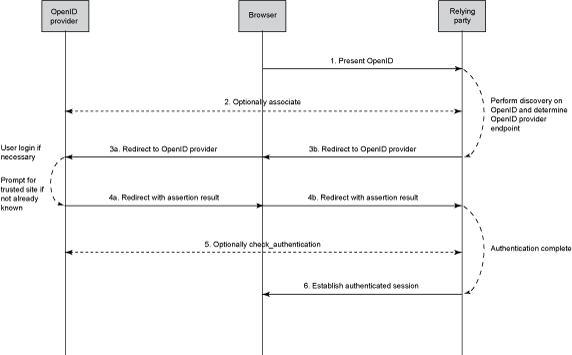
\includegraphics[scale=0.6]{picture/openid-flow.png}
\caption{OpenID overview}
\end{figure}

\section{Existing Solutions}

Since researchers have studied authentication system for years, there are various of solution now. I selected four kinds of solution, which is related to hardware-token, mobile device and smart card. These features are similar to the scheme I proposed. I describe them briefly in the following section.

\subsection{Token-based scheme}

\subsubsection{SecurID}

SecurID, now known as RSA SecurID, is a mechanism developed by RSA (the Security Division of EMC) for performing two-factor authentication for a user to a network resource. The following paragragh will describe how it works simply.

Each device stored a defferent secret \emph{seed}, and the back-end server also know this seed. In every 60 seconds, SecurID will generate an 6-digit authentication code according to its seed, and display on the screen. If a user authenticating to a network service, he have to enter both a personal identificaiton number and the 6-digit \emph{code at that moment}. The server, which also has a real-time clock and a database of valid tokens with the associated seed records, authenticates a user by computing what number the token is supposed to be showing at that moment in time and checking this against what the user entered.

However, in March 2011 attackers compromised RSA's back-end database of seeds, which allowed them to predict the authentication codes generated by any token at any time. This attack forces RSA Security to replace almost every one of the 40 million SecurID tokens in use.

\subsubsection{YubiKey}

The YubiKey is another authentication hardware token, which shaped like a USB flash drive. It connects to a USB port and identifies itself as a USB keyboard, which allows it to be compatiable to most of computers or laptops with system's native driver. The basic finction of the YubiKey is to generate \emph{One-Time Passwords}. 

When users want to authenticating to a network service by YubiKey, after insert YubiKey into the USB port, users have to touch the YubiKey's OTP generation button. The YubiKey will help users typing a string of printable characters-the concatenation of a fixed \emph{identity string} (replacing the username) and a one-time password (replacingthe password). Then the verify server will check whether the OTP is valid or not, and check the timestamp to resist to the relay-attak.

\subsection{Mobile-device-based scheme}

\subsubsection{Google 2-step}

Two-step verification is a process involving two stages to verify the identity of an entity trying to access services in a computer or in a network. Google was one of the first Internet companies to introduce a two-step verification process. The first authentication step is just like the original scheme, log in with the username and password. The second step required a mobile phone with SMS service. Users must register his phone number to Google. When a user want to start the 2-step authentication, a text message, which including a one-time code, will send to user's mobile phone via SMS. The user have to enter this code on the website in 30 seconds, or this code will be invalid because of timeout.

\subsection{Smart-card-based scheme}

\subsubsection{Swarn's Smart-card-based Scheme}

\end{CJK}
\begin{CJK}{Bg5}{bsmi}

%---------------------------------------------
%	Chapter System Architecture
%---------------------------------------------

\chapter{System Architecture}

In this chapter, I'll try to explain my design more detailed. First section is the basic idea of my authentication system, which is based on digital signature algorithm. The next section is about the flow if clinets and servers adopt this scheme. The next chapter gives two demonstrations of this scheme. One is for the furture website, and one if for the existing website. The last section gives a high-level code example to explain how to implement this system.

\section{Overview}

Let us recall the autehentication process about password-based scheme. As the fig\ref{fig:password-based-flow} shows, the client give his username and password to server (password is encrypted), and the server checks whether it is valid according to its database. Fig\ref{fig:my-scheme-flow} is the authentication process of my scheme. Because the verificaiton server should be a passive element, client should send a login request first. After receive a login request, the server send a random nonce back to client. Client generate a signature for this nonce and return to server. Server, then, use the public key to check whether the client is valid or not.

\begin{figure}
\centering
\subfigure[password-based scheme]{
\label{fig:password-based-flow}
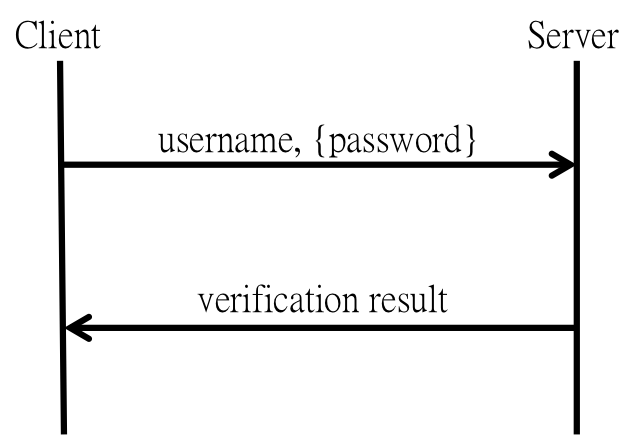
\includegraphics[scale=0.6]{picture/password-based-flow.png}
}
\subfigure[my scheme]{
\label{fig:my-scheme-flow}
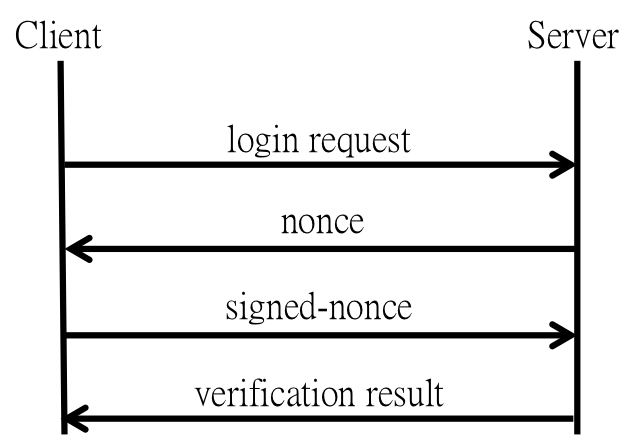
\includegraphics[scale=0.6]{picture/basic-idea-flow.png}
}
\caption{Authentication flow}
\end{figure}

This is how I used Digital Signature Algorithms in an authentication process. The advantages is that the data communicated between client and server do not need to be encrypted. The only \emph{secret} is private key, which is stored in client's storage. The disavantage of my scheme is that users will need a device to help them creating signature and manage their public keys. Therefore, the use of mobile device is the core of this scheme, bring us a high usability. The user flow become fig\ref{final-flow} with the help of mobile device.

\begin{figure}
\centering
\label{fig:final-flow}
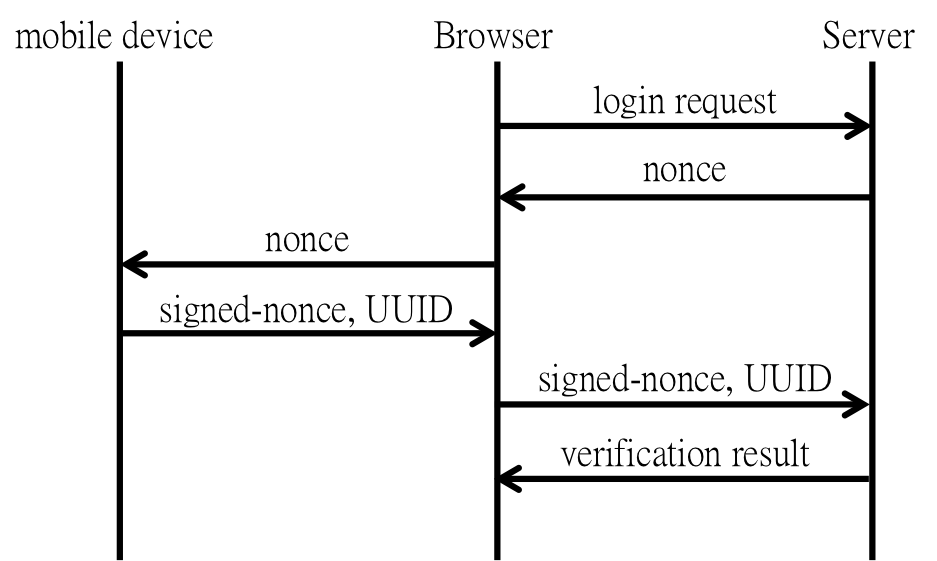
\includegraphics[scale=0.65]{picture/final-flow.png}
\caption{Authentication flow with mobile device}
\end{figure}

\section{User Flow}

In this section, I'll seperate the autentication process into three parts: \emph{register phase}, \emph{login phase} and \emph{verification phase}.

\subsubsection{Register Phase}

\begin{enumerate}
\item Start the initialzization process on his mobile device, that is, set PIN code and generate key pair.
\item User send a registration request to the verification server.
\item Server return the server information to user and pass it to mobile device via reader applicaiton.
\item Mobile device saved the server information and the private key together, and return the device UUID and corresponding public key back to user.
\item User send the id and public key (and other required credentials required by server) to server.
\item Server saved UUID and public key into its database.
\end{enumerate}

\subsubsection{Login Phase}

	1. User send a login requesr to server

	2. Server return a nonce ({server info || randombits}) back to browser

	3. The brower pass this nonce to reader application
		i.	The reader start to scan NFC cards.
		ii.	Timeout: 30 seconds

	4. Mobile device ask user to input the correct PIN code and confirm the server information
		i.	Enable card emulation mode right after receive correct PIN code

	5. Mobile device get nonce from reader application
		i.	mobile device signed the nonce with correspond private key.
		ii.	mobile device return the signed-nonce back to reader application

	6. Reader application return signed-nonce back to server.

\subsubsection{Verification Phase}

	1. Server find the corresponding public key accordding to id.

	2. Verify the signature.

	3. Return the result.

\section{Scenario}

\subsection{Future Website}

\subsection{Existing Website}

\section{Implementation}

\end{CJK}
\begin{CJK}{Bg5}{bsmi}

%---------------------------------------------
%	Chapter Discussion
%---------------------------------------------

\chapter{Discussion}

\section{Security Analysis}

\begin{comment}
This is the most important part of an authentication system.
We have to define our threat model before we start to analyze.
There are 4 components in the scheme I proposed.
\end{comment}

\subsection{Threat Model}

\subsection{Analysis}

\section{Usability Analysis}

\begin{comment}
The usability can not be neglected when researchers trying to design a system.
Usability is a subjective perception, it may be different from person to person.
The following paragragh states the criterias I used to estimate the usability of a system.
\end{comment}

\section{Deployment Ability Analysis}

\begin{comment}
The deployment ability is also an important thing which is need to be considered, especially in designing an authentication system.
A system with high usability means it is friendly to users; a system with high deployment ability means it is friendly to the system provider or, more precise, the developers.
The following paragraph states the criterias I used to estimate a system's deployment ability. 
\end{comment}


\end{CJK}
\begin{CJK}{Bg5}{bsmi}

%---------------------------------------------
%	Chapter Conclusion
%---------------------------------------------

\chapter{Conclusion}

\section{Compare to Other Schemes}

\end{CJK}

\printindex


\bibliographystyle{alpha}
\bibliography{cloudgpuenum}


\end{document}